\documentclass{beamer}
\usetheme[pageofpages=of,% String used between the current page and the
                         % total page count.
          bullet=circle,% Use circles instead of squares for bullets.
          titleline=true,% Show a line below the frame title.
          alternativetitlepage=true,% Use the fancy title page.
       %   titlepagelogo=logo-polito,% Logo for the first page.
       %   watermark=watermark-polito,% Watermark used in every page.
       %   watermarkheight=100px,% Height of the watermark.
       %   watermarkheightmult=4,% The watermark image is 4 times bigger
                                % than watermarkheight.
          ]{Torino}

\setbeamertemplate{footline}{
  \begin{beamercolorbox}[wd=\paperwidth,ht=1ex,dp=1ex]{footline}
    \vspace{5pt} \hspace{1em} \insertframenumber/\inserttotalframenumber
  \end{beamercolorbox}
}

\author{Brendon J. Brewer}
\title{STATS 331 -- Introduction to Bayesian Statistics}
\institute{The University of Auckland}
\date{}


\linespread{1.3}
\usepackage{minted}
\usepackage[utf8]{inputenc}
\usepackage{dsfont}
\newcommand{\given}{\,|\,}

\begin{document}

\frame{\titlepage}

\begin{frame}
\begin{center}
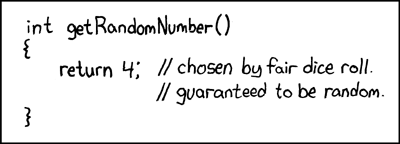
\includegraphics[width=0.6\textwidth]{images/random_number.png} \\

Credit: Randall Monroe, xkcd.com
\end{center}

\end{frame}

\begin{frame}
\begin{center}
\Large
Introduction to JAGS
\end{center}
\end{frame}


\begin{frame}
\frametitle{Introduction to JAGS}

\begin{itemize}
\item JAGS is a general purpose computer program for doing
MCMC sampling.\pause
\item It is useful for routine analyses (less useful for very large or
research problems).\pause
\item You tell it the prior, the sampling distribution, and the data and it will
do everything for you!\pause
\item It uses methods other than Metropolis (Gibbs sampling,
slice sampling, ...).
\end{itemize}

\end{frame}


\begin{frame}
\frametitle{Alternatives to JAGS}

There are some other programs similar to JAGS. I will mention them here,
so that you've heard of them, but we will not use them in this course.

\begin{itemize}
\item WinBUGS and OpenBUGS are both very similar to JAGS (the former is very
old and only works on Microsoft Windows).
Most of the time, code would not need to be modified to work in any of these.\pause
\item {\bf Stan} is a more modern and very popular package. It uses similar
ideas to JAGS, but its language is a bit different, and it uses a different,
more complex
MCMC sampler (based on {\bf Hamiltonian Monte Carlo}).
\end{itemize}

\end{frame}

\begin{frame}[fragile]
\frametitle{Installing JAGS}
You can install JAGS by first downloading it from this URL. Install it to
the default location on your system to avoid problems later.

\begin{center}
\url{https://mcmc-jags.sourceforge.io/}
\end{center}

\pause

After installing JAGS itself, you should install the \mintinline{r}{rjags}
package inside R:
\begin{minted}{r}
install.packages("rjags")
\end{minted}

\end{frame}


\begin{frame}[fragile]
\frametitle{The Bus Problem}
Recall the bus problem from the lecture notes. This was a binomial experiment
with $N=5$ trials, and the data was $x=2$ successes. The unknown parameter
is $\theta$, the success probability that applies on each trial.

\pause

We know how to solve this with a grid (Bayes Box), analytically (with a Beta
or Uniform prior for $\theta$), and with Metropolis.
How would we implement this in JAGS?

\end{frame}


\begin{frame}[fragile]
\frametitle{The Bus Problem in JAGS}

\begin{minted}{r}
model
{
    # The prior for the parameter
    theta ~ dunif(0, 1)

    # Sampling distribution (prior for the data!)
    x ~ dbin(theta, N)
}
\end{minted}

\end{frame}

\begin{frame}[fragile]
\frametitle{The Bus Problem in JAGS}
\begin{itemize}
\item We always write the assumptions inside the \mintinline{r}{model} block.\pause
\item We generally put the prior before the sampling distribution, but we don't
    actually have to!\pause
\item Quantities (either parameters or data) are defined into existence using
the tilde \mintinline{r}{~}.\pause
\item Note that $N$ is not defined anywhere --- this will be provided along
with the data value $x$.
\end{itemize}

\end{frame}

\begin{frame}[fragile]
\frametitle{Note About dbin() in JAGS}

\begin{itemize}
\item The distributions in JAGS are named similarly to the \mintinline{r}{d}
(density) functions in R, but not exactly the same --- here we see
\mintinline{r}{dbin()} whereas in R it's \mintinline{r}{dbinom()}.\pause
\item Also, people usually write Binomial$(N, p)$ or Binomial$(N, \theta)$,
but in JAGS the arguments are the other way around.\pause
\item There are some other quirks. E.g., for the normal distribution, the
second argument is {\em one over the variance}, i.e., we must write
\mintinline{r}{dnorm(mu, 1/sigma^2)}. 
We could write \mintinline{r}{dnorm(mu, 5)}
but the meaning of the second parameter is obscured.
\end{itemize}

\end{frame}



\begin{frame}[fragile]
\frametitle{Running JAGS from R}

\begin{itemize}
\item We will write R code that calls JAGS in the background using functions
from the \mintinline{r}{rjags} package.\pause
\item There is a script on Canvas called \texttt{use\_jags.R} which you can
use as a template.\pause
\item The JAGS model code is provided inside an R string.\pause
\item The data must be in an R list or data frame.\pause
\item After running the script, the results are put into a data frame called
\mintinline{r}{results}, whose (named) columns are the parameters.
\end{itemize}

\end{frame}

\begin{frame}
\frametitle{R Lists}
In case anyone here has programmed in another
language before:
\begin{itemize}
\item An R list is like a C/C++ struct, or a Java class with no methods.\pause
\item An R list is like a Python dictionary.
\end{itemize}

\pause
A list contains multiple objects which may be of different types, and may be
named.
\end{frame}

\begin{frame}[fragile]
\frametitle{R List Example}
\begin{minted}{r}
> me = list(name="Brendon", age=30 + 20*runif(1))
> me
$name
[1] "Brendon"

$age
[1] 43.22408
\end{minted}
(not accurate)
\end{frame}


\begin{frame}[fragile]
\frametitle{Accessing List Elements}
List elements can be accessed by name using the dollar sign
or by number using double square brackets.
\begin{minted}{r}
> me$name
[1] "Brendon"
> me$age
[1] 43.22408
> me[[1]]
[1] "Brendon"
> me[[2]]
[1] 43.22408
\end{minted}
\end{frame}


\begin{frame}[fragile]
\frametitle{Uses for R lists}
\begin{itemize}
\item R Lists are useful for organising data/variables that
belong together into a single ``object''.\pause
\item Also, for being able to return more than one result from
a function --- just pack it all into a list before the
\mintinline{r}{return} statement.
\end{itemize}

\pause
When running JAGS, we will often put the data into a list.
E.g. for the bus problem,
\begin{minted}{r}
data = list(x=2, N=5)
\end{minted}
\end{frame}


\begin{frame}[fragile]
\frametitle{Running JAGS on the Bus Problem}
Let's run JAGS on the bus problem. We will need to ``monitor''
\mintinline{r}{theta}, by including it in the \mintinline{r}{variable_names}
vector, if we want to see it in the output.

\end{frame}



\begin{frame}[fragile]
\frametitle{Visualisation and Summaries}
It is easy to visualise and summarise the posterior:

\begin{minted}{r}
plot(results$theta, type=”l”)
hist(results$theta, breaks=100)
mean(results$theta)
sd(results$theta)
\end{minted}

\end{frame}



\begin{frame}[fragile]
\frametitle{Coal Data}

\centering
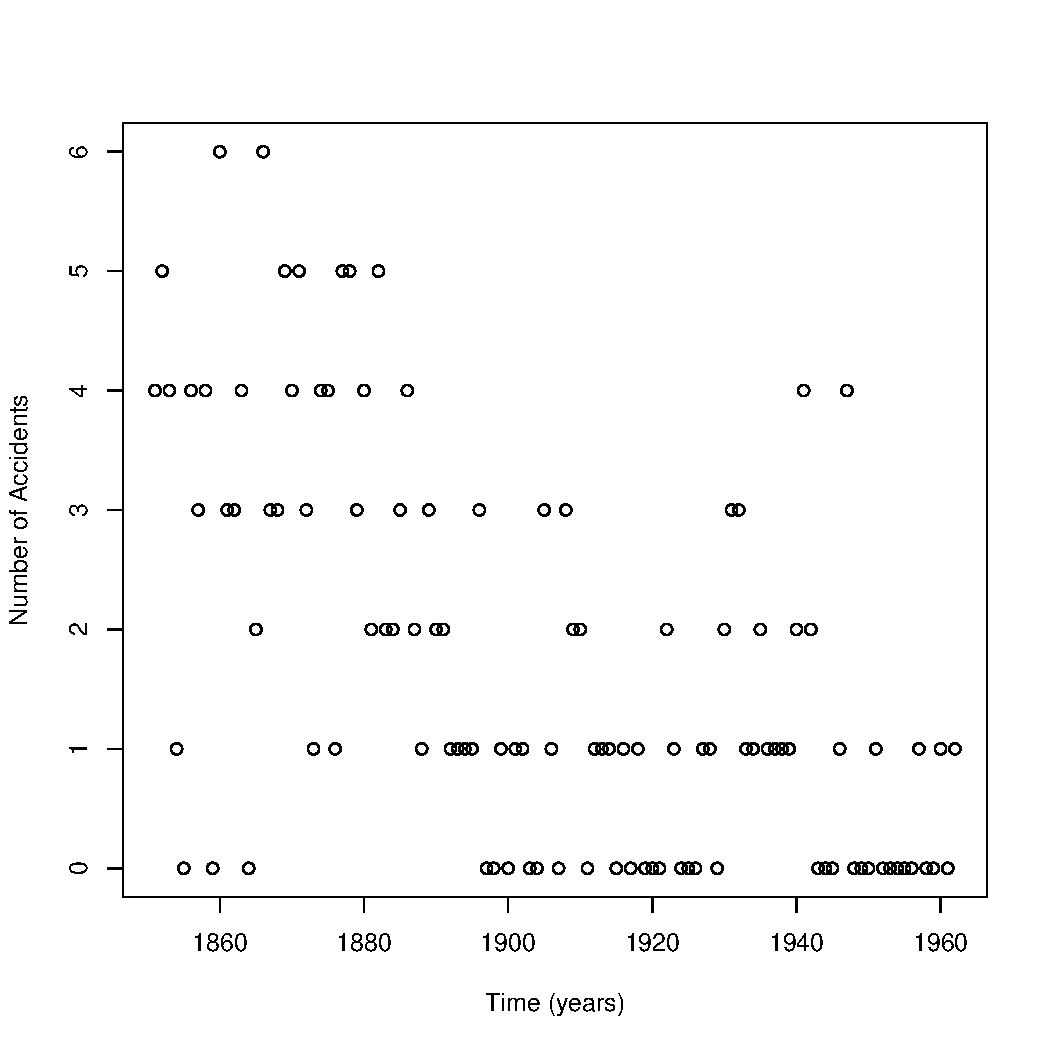
\includegraphics[width=0.6\textwidth]{images/coal.pdf}

\end{frame}


\begin{frame}[fragile]
\frametitle{Coal Data}
The coal mining data is in a .R file that just defines a list.
We need to ``source'' the file --- run all the code in it. We can just
click source in RStudio, or we can use the \mintinline{r}{source()}
function to do it:
\begin{minted}{r}
source("coal.R")
\end{minted}
\pause
We may need to put the full file path in the argument, or change
R's working directory.

\end{frame}




\begin{frame}[fragile]
\frametitle{Coal Mining Accidents --- Simple Model}

\begin{minted}{r}
model
{
    # Somewhat arbitrary upper limit
    lambda ~ dunif(0, 1000)

    for(i in 1:N) # For-loop syntax is like R
    {
        y[i] ~ dpois(lambda)
    }
}
\end{minted}

\end{frame}


\begin{frame}[fragile]
\frametitle{Coal Mining Accidents --- For Loop}
\begin{itemize}
\item The sampling distribution involves a loop because we have a vector
of data values.\pause
\item This is usually what happens, but not always --- it is possible to
put parameters in a vector too, if you want.\pause
\item The for-loop syntax is very similar to R's for loops.\pause
\item \mintinline{r}{N}, the number of data points, is defined in the
data list. We could also use \mintinline{r}{for(i in 1:length(y))} or
\mintinline{r}{for(i in 1:length(t))}.
\end{itemize}

\end{frame}


\begin{frame}[fragile]
\frametitle{Coal Mining Accidents --- Results}
Let's run \texttt{use\_jags.R} and look at the results.

\end{frame}



\begin{frame}
\frametitle{Coal Mining Accidents --- Log-Uniform Prior}
We will now see how to define a log-uniform prior in JAGS,
as an alternative to the Uniform$(0, 1000)$ prior that we have
seen so far. Remember, there are two ways of defining the
log-uniform prior:\pause
\begin{align}
p(\lambda) &\propto 1/\lambda, \quad \lambda > 0
\end{align}
\pause
or
\begin{align}
\log \lambda &\sim \textnormal{Uniform}(-\infty, \infty).
\end{align}
\pause
JAGS doesn't allow infinite range (an `improper' prior),
but we can just use a wide range.

\end{frame}


\begin{frame}[fragile]
\frametitle{Coal Mining Accidents --- Log-Uniform Prior}
To define a log-uniform prior in JAGS, we can use two lines of code.
\begin{minted}{r}
log_lambda ~ dunif(-10, 10)
lambda <- exp(log_lambda)
\end{minted}
\pause

The first line creates a parameter with a uniform prior. If
we exponentiate it, the result has a log-uniform prior.\pause

The range is from $e^{-10} \approx 0.000045$ to $e^{10} \approx 22000$,
which is wide enough for most purposes. Not astronomy though!
\end{frame}


\begin{frame}[fragile]
\frametitle{Deterministic and Stochastic Nodes}
\begin{itemize}
\item The parameter \mintinline{r}{lambda} was defined using \mintinline{r}{<-}
using an equation, not a probability distribution. Because an equation always
gives a definite answer, this is called a {\em deterministic node}. \pause
\item Quantities defined using \mintinline{r}{~} and a probability distribution,
whether they are parameters or data values, are called
{\em stochastic nodes}.
\end{itemize}
\end{frame}


\begin{frame}[fragile]
\frametitle{Coal Mining Accidents --- ChangePoint Model}
We will now make a more complicated model, to show the power of JAGS and
MCMC. It will be a
``change-point'' model, where instead of having a
constant $\lambda$ value, we assume it changes from
$\lambda_1$ to $\lambda_2$ at some critical time $t_c$.
These are the three unknown parameters.

Looking at the data, something like this might be going on.
\end{frame}

\begin{frame}[fragile]
\frametitle{Coal Data}

\centering
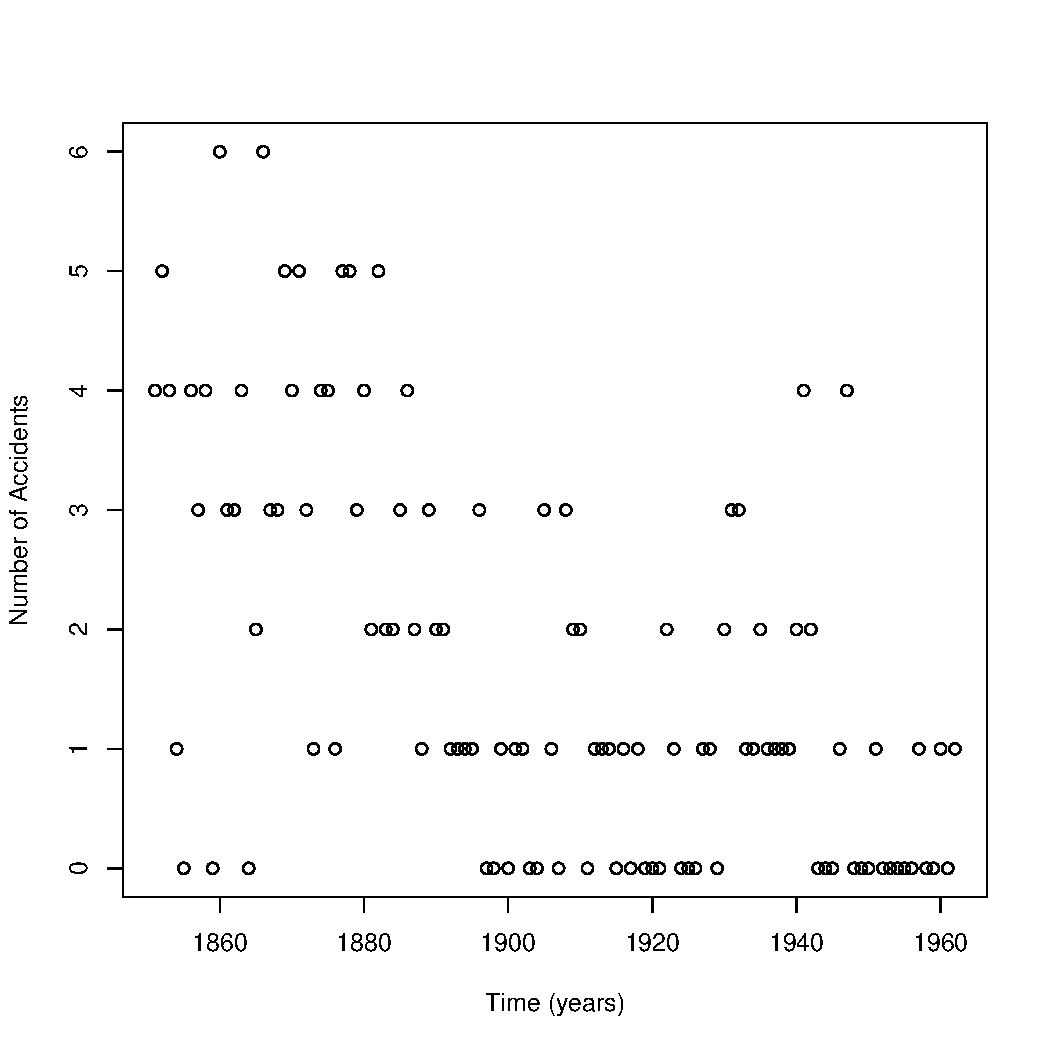
\includegraphics[width=0.6\textwidth]{images/coal.pdf}

\end{frame}


\begin{frame}[fragile]
\frametitle{Change-Point Model: Priors}
We will use log-uniform priors for $\lambda_1$ and $\lambda_2$ independently.
\begin{minted}{r}
log_lambda1 ~ dunif(-10, 10)
lambda1 <- exp(log_lambda1)

log_lambda2 ~ dunif(-10, 10)
lambda2 <- exp(log_lambda2)
\end{minted}
\pause
Note: Distributions will be independent if, when defining one, you
make no reference to another node on the right hand side.

\end{frame}

\begin{frame}[fragile]
\frametitle{Change-Point Model: Priors}
We will use a uniform prior for the change year, $t_c$, between the
endpoints of the data.
\begin{minted}{r}
t_c ~ dunif(1851, 1962)
\end{minted}
\pause

{\bf Note:}
While it might look like we are defining a prior based on the data,
which is not technically valid, we are actually not. The time values
in the data are prior information, not data, as they have no sampling
distribution --- our whole calculation is conditional on it already.

\end{frame}


\begin{frame}[fragile]
\frametitle{Change-Point Model: Sampling Distribution}
To construct the sampling distribution we will use \mintinline{r}{step()}
which is like R's \mintinline{r}{ifelse()}. It returns 0 if the argument is
negative and 1 otherwise.

\begin{minted}{r}
for(i in 1:N)
{
    mu[i] <- lambda1 + step(t[i] - t_c)*(lambda2 - lambda1)
    y[i] ~ dpois(mu[i])
}
\end{minted}
\pause

We could have done this in one line, without defining \mintinline{r}{mu}
first.

\end{frame}



\end{document}

